\documentclass[a4paper]{article}

\usepackage[francais]{babel}
\usepackage[T1]{fontenc}
\usepackage[utf8]{inputenc}
\usepackage{algorithm}
\usepackage[end]{algpseudocode}
\usepackage{graphicx}

\title{Tests sur les différentes topologies avec 4 LoPy}

\author{Olivier Flauzac, Hérard Joffrey}

\date{\today}

\begin{document}
\maketitle
\begin{enumerate}
\item 1 \textit{LWGW}, 1 \textit{LGW}, 1 \textit{IN} 

\item 1 \textit{LWGW}, 1 \textit{LGW}, k \textit{IN}  
	\begin{itemize}
		\item  1 \textit{LWGW}, 1 \textit{LGW}, 2 \textit{IN}  
		\item  1 \textit{LWGW}, 1 \textit{LGW}, 3 \textit{IN}  
	\end{itemize}

\item 1 \textit{LWGW}, k \textit{LGW} , k \textit{IN}  
	\begin{itemize}
		\item  1 \textit{LWGW}, 2 \textit{LGW}, 1 \textit{IN}  
		\item  1 \textit{LWGW}, 2 \textit{LGW}, 2 \textit{IN}  
	\end{itemize}
\end{enumerate}

\newpage
\section{ 1 \textit{LWGW} <->, 1 \textit{LGW} <-> 1 \textit{IN} }
\begin{figure}[h!]
\centering
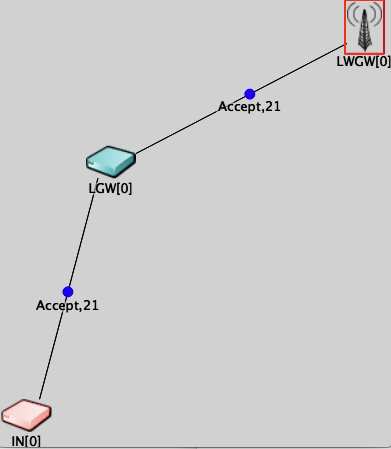
\includegraphics[scale=0.5]{../Rapport_PFE/chaine.png} 
\end{figure}
\newpage
\section{ 1 \textit{LWGW} <->, 1 \textit{LGW} <-> K \textit{IN} }
\subsection{ 1 \textit{LWGW} <->, 1 \textit{LGW} <-> 2 \textit{IN} }
\begin{figure}[h!]
\centering
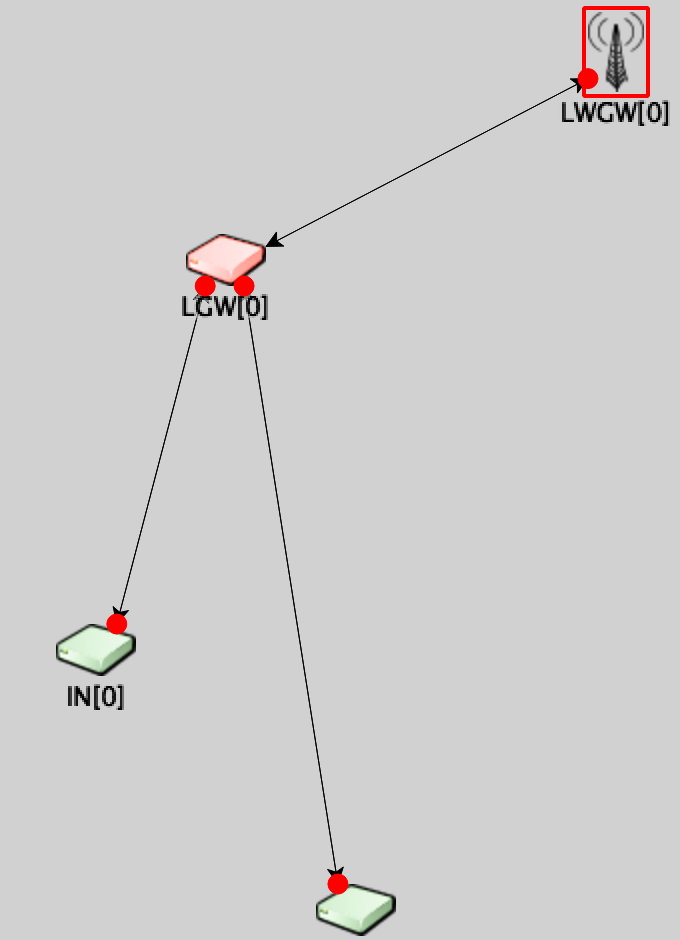
\includegraphics[scale=0.5]{cas_2.png} 
\end{figure}
\newpage

\subsection{ 1 \textit{LWGW} <->, 1 \textit{LGW} <-> 2 \textit{IN} avec interconnexions }
\begin{figure}[h!]
\centering
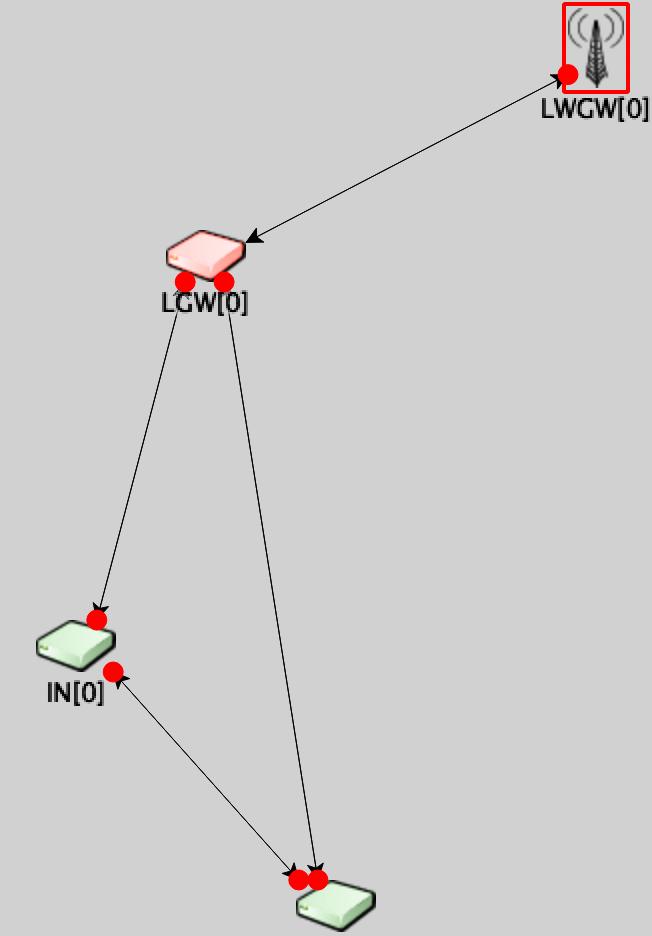
\includegraphics[scale=0.5]{cas_2_1.png} 
\end{figure}

\newpage
\subsection{ 1 \textit{LWGW} <->, 1 \textit{LGW} <-> 3 \textit{IN} }
\begin{figure}[h!]
\centering
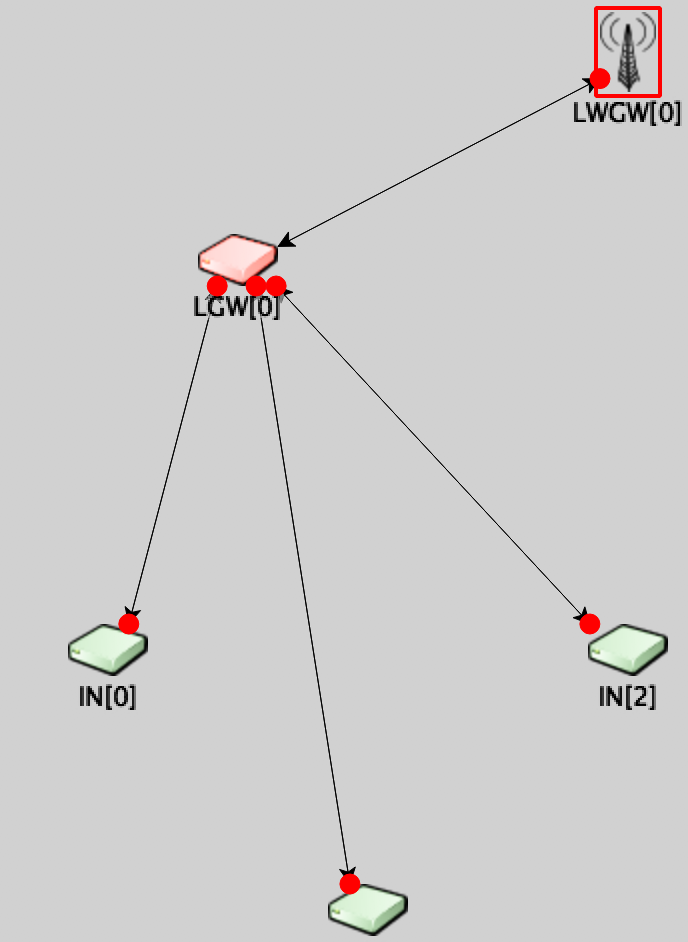
\includegraphics[scale=0.5]{cas_3.png} 
\end{figure}


\newpage
\subsection{ 1 \textit{LWGW} <->, 1 \textit{LGW} <-> 3 \textit{IN} avec 2 interconnexions entre IN}
\begin{figure}[h!]
\centering
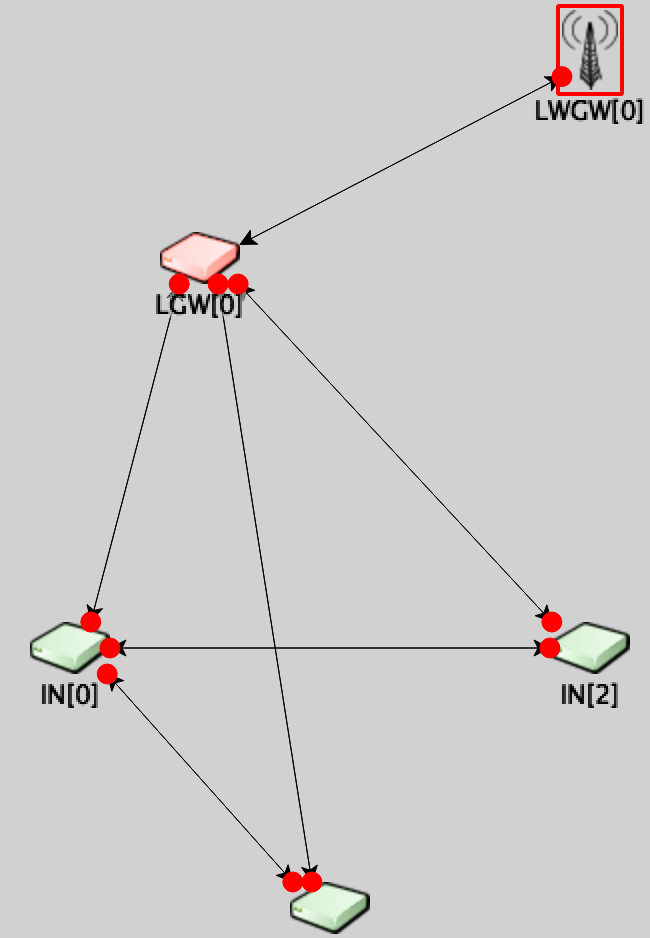
\includegraphics[scale=0.5]{cas_3_1.png} 
\end{figure}


\newpage
\subsection{ 1 \textit{LWGW} <->, 1 \textit{LGW} <-> 3 \textit{IN} avec une Clique entre les INs }
\begin{figure}[h!]
\centering
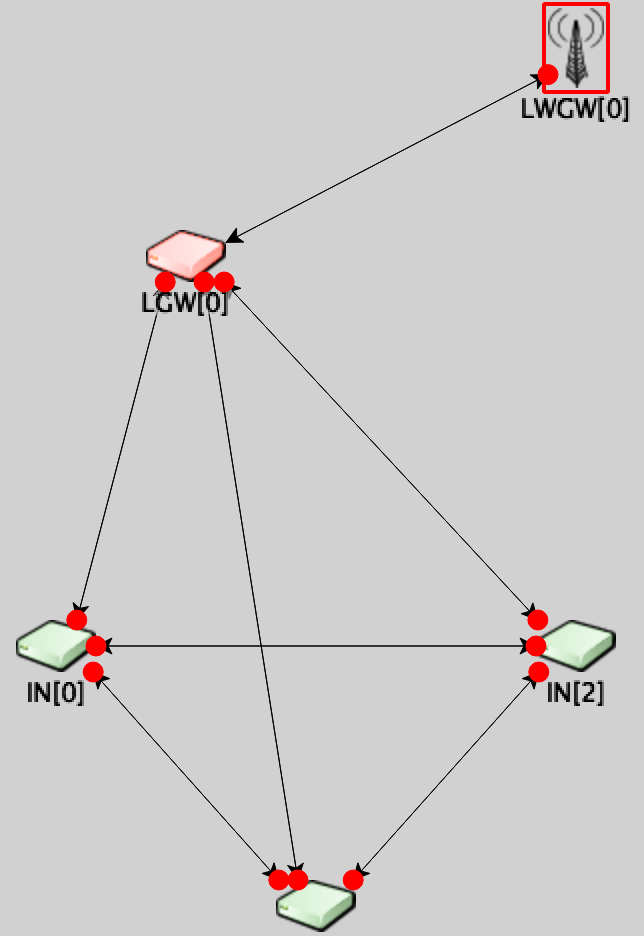
\includegraphics[scale=0.5]{cas_3_2.png} 
\end{figure}


\newpage
\section{ 1 \textit{LWGW} <->, 2 \textit{LGW} <-> 2 \textit{IN} }
\subsection{ 1 \textit{LWGW} <->, 1 \textit{LGW} <-> 3 \textit{IN} avec 0 interconnexion entre IN}
\begin{figure}[h!]
\centering
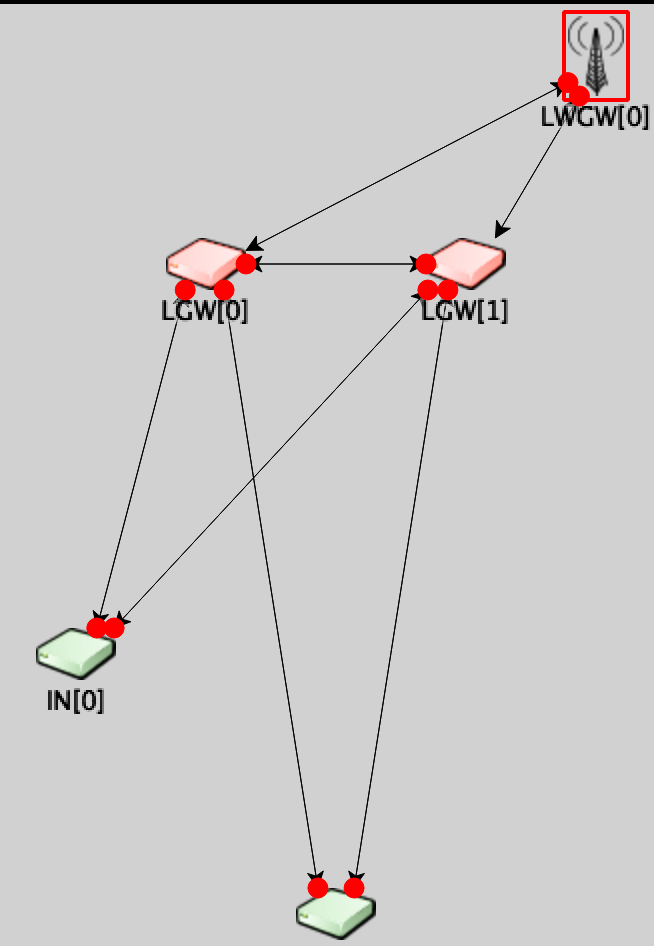
\includegraphics[scale=0.5]{cas_1.png} 
\end{figure}
\newpage
\subsection{ 1 \textit{LWGW} <->, 1 \textit{LGW} <-> 3 \textit{IN} avec interconnexions entre IN}
\begin{figure}[h!]
\centering
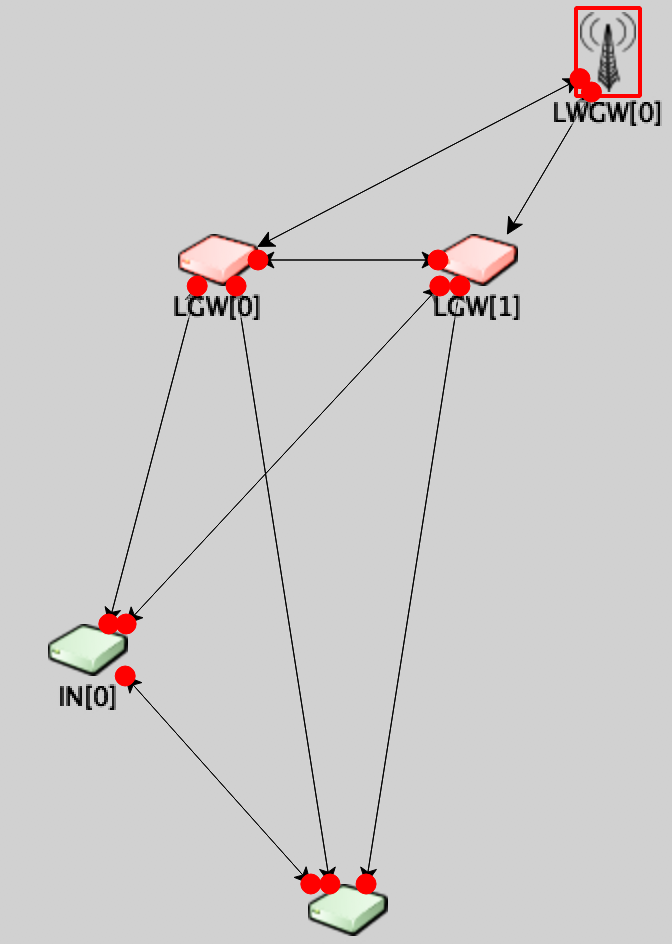
\includegraphics[scale=0.5]{cas_1_1.png} 
\end{figure}

\end{document}
